\PassOptionsToPackage{table}{xcolor}

\documentclass[
%	handout,
	notes=none,
	aspectratio=169
]{beamer}

% Comment out the following line to hide the notes
%\setbeameroption{show notes}

\input{macros}

\usefolder{theme}
\usetheme{TuringDark}

\begin{document}

\title{Tutorial 3: Multi-node training with Lightning}
\subtitle{Converting GPT2 to use MPI and Lightning}
\author{HPC Training -- 25-26 November 2025 \\David Llewellyn-Jones}
%\date{30 January 2025}

%%%%%%%%%%%%%%%%%%%%%%%%%%%%%%%%%%%%%%%%%

\renewcommand{\thefootnote}{\arabic{footnote}}

\frame{
\titlepage
}
\note{
}

\renewcommand{\thefootnote}{\fnsymbol{footnote}}

%%%%%%%%%%%%%%%%%%%%%%%%%%%%%%%%%%%%%%%%

\begin{frame}
\frametitle{Motivation}

\begin{columns}[T]
\begin{column}[T]{1.0\textwidth}
\setlength{\parskip}{0.5em}

\vspace{-0.5cm}
GPUs are great for accelerated training and inference, but processing is bounded by:
\begin{enumerate}
\setlength{\parskip}{0.5em}
\item Available memory
\item Speed of computation
\end{enumerate}
How to make AI better?
\begin{enumerate}
\item Improved algorithms
\item Larger models
\item More training data
\end{enumerate}
The last two require {\it more compute}

\end{column}
\end{columns}

\end{frame}
\note{
}

%%%%%%%%%%%%%%%%%%%%%%%%%%%%%%%%%%%%%%%%%

\begin{frame}
\frametitle{Scaling up}

\begin{columns}[T]
\begin{column}[T]{1.0\textwidth}
\setlength{\parskip}{0.5em}

\vspace{-0.5cm}
\begin{enumerate}
\setlength{\parskip}{0.5em}
\item Strong motivation for scaling across GPUs
\item Single device: 4 or 8 GPUs maximum
\item Eventually want to scale across nodes
\item Get this right... the sky's the limit
\end{enumerate}

\end{column}
\end{columns}

\end{frame}
\note{
}

%%%%%%%%%%%%%%%%%%%%%%%%%%%%%%%%%%%%%%%%%

\begin{frame}
\frametitle{Preparation}

\begin{columns}[T]
\begin{column}[T]{0.52\textwidth}
\setlength{\parskip}{0.5em}

\vspace{0.0cm}
\begin{enumerate}
\setlength{\parskip}{0.5em}
\item Open Baskerville docs\\\url{https://docs.baskerville.ac.uk}
\item Select \href{https://portal.baskerville.ac.uk/}{Baserville Portal}
\item Login if necessary
\item Select \href{https://portal.baskerville.ac.uk/pun/sys/dashboard/batch_connect/sys/bc_bask_jupyter/session_contexts/new}{JupyterLab} Apps list
\item Configure the session
\item Launch
\end{enumerate}
\end{column}

\begin{column}[T]{0.48\textwidth}
\vspace{-0.1cm}
\begin{tcolorbox}[colback=slidebg,colframe=cyan!50!black,title=Session configuration]
\small
\begin{enumerate}
\setlength{\parskip}{0.5em}
\item Kernel: {\tt Python 3.11.3}
\item Show Conda Envs: {\tt No}
\item Number of hours: {\tt 2}
\item Number of GPUs: {\tt 1}
\item Project: {\tt vjgo8416-hpc2511}
\item Queue: {\tt turing}
\end{enumerate}
\end{tcolorbox}
\end{column}

\end{columns}

\end{frame}
\note{
}

%%%%%%%%%%%%%%%%%%%%%%%%%%%%%%%%%%%%%%%%%

\begin{frame}
\frametitle{}

\begin{columns}[T]
\begin{column}[T]{1.0\textwidth}
\setlength{\parskip}{0.5em}

\vspace{0.0cm}
\includegraphics[width=1.0\textwidth]{launch-jupyterlab}


\end{column}
\end{columns}

\end{frame}
\note{
}

%%%%%%%%%%%%%%%%%%%%%%%%%%%%%%%%%%%%%%%%%

\begin{frame}
\frametitle{Data parallel}

\begin{columns}[T]
\begin{column}[T]{0.9\textwidth}
\setlength{\parskip}{0.5em}

\vspace{-0.5cm}
\includegraphics[width=1.0\textwidth]{parallel-data}


\end{column}
\end{columns}

\end{frame}
\note{
}

%%%%%%%%%%%%%%%%%%%%%%%%%%%%%%%%%%%%%%%%%

\begin{frame}
\frametitle{Model parallel FSDP}

\begin{columns}[T]
\begin{column}[T]{0.7\textwidth}
\setlength{\parskip}{0.5em}

\vspace{-1.5cm}
\includegraphics[width=1.0\textwidth]{parallel-vertical}


\end{column}
\end{columns}

\end{frame}
\note{
}

%%%%%%%%%%%%%%%%%%%%%%%%%%%%%%%%%%%%%%%%%

\begin{frame}
\frametitle{The plan}

\begin{columns}[T]
\begin{column}[T]{0.7\textwidth}
\setlength{\parskip}{0.5em}

\vspace{0.0cm}
\begin{enumerate}
\setlength{\parskip}{0.5em}
\item No more theory
\item Simplified GPT2 nano code for one GPU
\item Andrej Karpathy: \url{https://youtu.be/l8pRSuU81PU}
\item Extend to support Distributed Data Parallel
\item Extend using PyTorch Lightning
\end{enumerate}

\end{column}
\begin{column}[T]{0.3\textwidth}
\setlength{\parskip}{0.5em}

\vspace{0.0cm}
\includegraphics[width=0.9\textwidth]{karpathy}

\end{column}
\end{columns}

\end{frame}
\note{
}

%%%%%%%%%%%%%%%%%%%%%%%%%%%%%%%%%%%%%%%%%

\begin{frame}
\frametitle{Your most important tools}

\begin{columns}[T]
\begin{column}[T]{0.7\textwidth}
\setlength{\parskip}{0.5em}

\vspace{0.0cm}
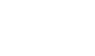
\includegraphics[width=1.0\textwidth]{tools}


\end{column}
\end{columns}

\end{frame}
\note{
}

%%%%%%%%%%%%%%%%%%%%%%%%%%%%%%%%%%%%%%%%%

\begin{frame}
\frametitle{Training terminology}

\begin{columns}[T]
\begin{column}[T]{1.0\textwidth}
\setlength{\parskip}{0.5em}

\vspace{0.0cm}
\begin{enumerate}
\setlength{\parskip}{0.0em}
\item Vocabulary: 50257 embeddings
\item Dataset: 9799991296 FineWeb tokens, our training data
\item Sample: a sequence of 1024 tokens from the dataset
\item Microbatch: 16 samples
\item Minibatch (also called a batch): 32 microbatches, gradient accumulation performed afterwards
\item Step: the process for training on one minibatch
\item Epoch: one training sweep of the entire dataset, 18692 steps
\end{enumerate}
\vspace{0.3cm}
$
\qquad \qquad 18692 \times 16 \times 32 \times 1024 = 9799991296
$

\end{column}
\end{columns}

\end{frame}
\note{
}

%%%%%%%%%%%%%%%%%%%%%%%%%%%%%%%%%%%%%%%%%

\begin{frame}
\frametitle{Training with 1 GPU}

\begin{columns}[T]
\begin{column}[T]{1.0\textwidth}
\setlength{\parskip}{0.5em}

\vspace{0.0cm}
\includegraphics[width=1.0\textwidth]{cadence-1gpu}


\end{column}
\end{columns}

\end{frame}
\note{
}

%%%%%%%%%%%%%%%%%%%%%%%%%%%%%%%%%%%%%%%%%

\begin{frame}
\frametitle{Training with 2 GPUs}

\begin{columns}[T]
\begin{column}[T]{1.0\textwidth}
\setlength{\parskip}{0.5em}

\vspace{0.0cm}
\includegraphics[width=1.0\textwidth]{cadence-2gpu}


\end{column}
\end{columns}

\end{frame}
\note{
}

%%%%%%%%%%%%%%%%%%%%%%%%%%%%%%%%%%%%%%%%%

\begin{frame}
\frametitle{Training with 4 GPUs}

\begin{columns}[T]
\begin{column}[T]{1.0\textwidth}
\setlength{\parskip}{0.5em}

\vspace{0.0cm}
\includegraphics[width=1.0\textwidth]{cadence-4gpu}


\end{column}
\end{columns}

\end{frame}
\note{
}

%%%%%%%%%%%%%%%%%%%%%%%%%%%%%%%%%%%%%%%%%

\begin{frame}
\frametitle{Distributed training terminology}

\begin{columns}[T]
\begin{column}[T]{1.0\textwidth}
\setlength{\parskip}{0.5em}

\vspace{0.0cm}
\begin{enumerate}
\setlength{\parskip}{0.5em}
\item Training on $n$ nodes, each with $m$ GPUs
\item Total $n \times m$ GPUs
\item World size: $w = m \times n$
\item Global rank $r_G$ is a unique index $r_G \in \{ 0, \ldots, w - 1 \}$
\item Local rank $r_L$ is unique per device $r_L \in \{ 0, \ldots, m - 1 \}$
\item No node index, but we do have {\it hostnames}, \eg\/ {\tt bask-pg0309u05a}, {\tt bask-pg0309u06a}
\item We may also have multiple CPU {\it workers\/} for each node
\end{enumerate}

\end{column}
\end{columns}

\end{frame}
\note{
}

%%%%%%%%%%%%%%%%%%%%%%%%%%%%%%%%%%%%%%%%%

\begin{frame}
\frametitle{Training with multiple nodes}

\begin{columns}[T]
\begin{column}[T]{1.0\textwidth}
\setlength{\parskip}{0.5em}

\vspace{0.0cm}
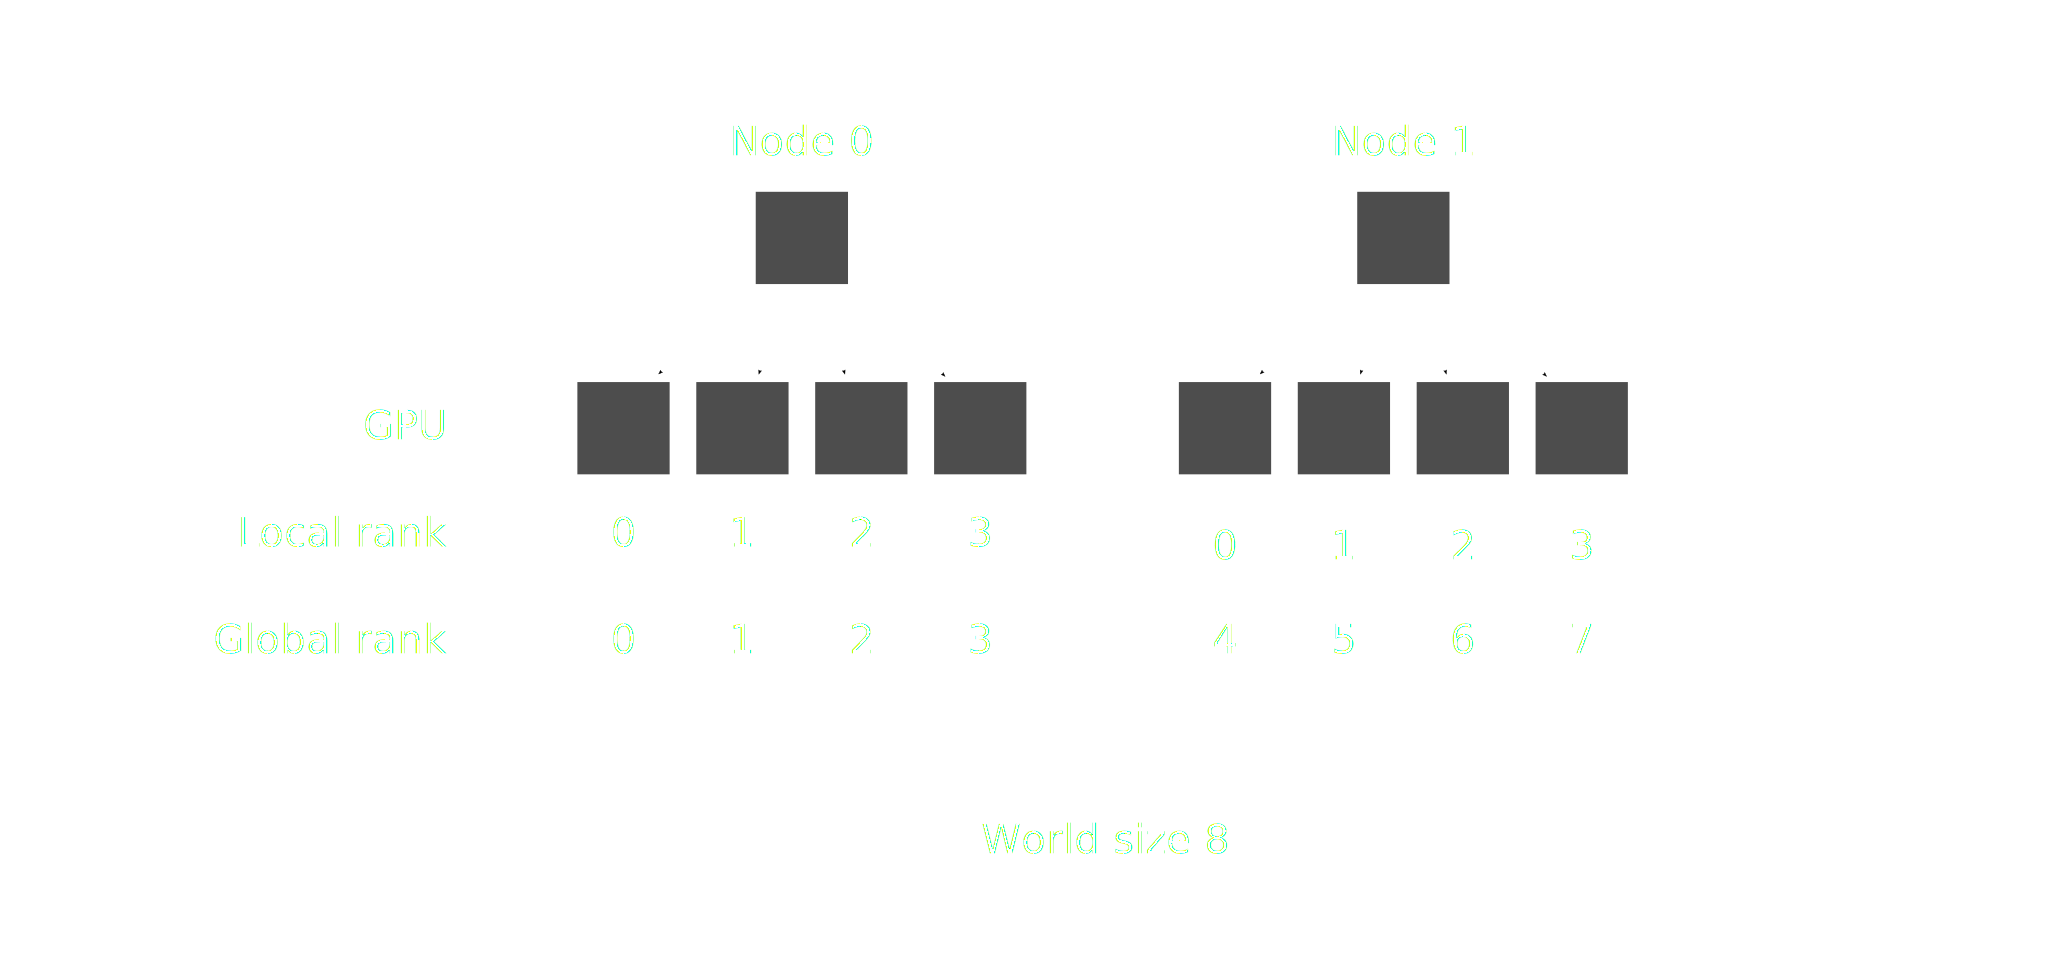
\includegraphics[width=1.0\textwidth]{world}


\end{column}
\end{columns}

\end{frame}
\note{
}

%%%%%%%%%%%%%%%%%%%%%%%%%%%%%%%%%%%%%%%%%

\begin{frame}[fragile]
\frametitle{Time to look at the code}

\begin{columns}[T]
\begin{column}[T]{1.0\textwidth}
\setlength{\parskip}{0.5em}

\vspace{-1.5cm}
\begin{enumerate}
\setlength{\parskip}{0.5em}
\item Open your JupyterLab page
\item Connect to Jupyter
\item Select the File Browser in the \\vertical bar on the left
\item Move to the directory: {\tt ~/vjgo8416-hpc2511/\$USER/hpc-training-nov-2025/3-Training/code}
\item Open the {\tt train\_gpt2.py} file by double-clicking on it
\end{enumerate}

\setlength{\parskip}{0.5em}

\vspace{-5.4cm}
\hfill
\includegraphics[width=0.45\textwidth]{connect-to-jupyter}

\end{column}
\end{columns}

\end{frame}
\note{
}

%%%%%%%%%%%%%%%%%%%%%%%%%%%%%%%%%%%%%%%%%

\begin{frame}
\frametitle{}

\begin{columns}[T]
\begin{column}[T]{1.0\textwidth}
\setlength{\parskip}{0.5em}

\vspace{0.0cm}
\includegraphics[width=1.0\textwidth]{traingpt2py}


\end{column}
\end{columns}

\end{frame}
\note{
}

%%%%%%%%%%%%%%%%%%%%%%%%%%%%%%%%%%%%%%%%%

\begin{frame}
\frametitle{GPT2 nano classes and functions}

\begin{columns}[T]
\begin{column}[T]{1.0\textwidth}
\setlength{\parskip}{0.5em}

\vspace{0.0cm}
\begin{enumerate}
\setlength{\parskip}{0.0em}
\item {\tt CausalSelfAttention}, {\tt MLP}, {\tt Block}: model components
\item {\tt GPTConfig}: model configuration
\item {\tt GPT}: the model
\item {\tt generate()}: inference
\item {\tt configure\_optimizers()}: training configuration
\item {\tt training\_step()}: one training step
\item {\tt load\_tokens()}: load a single FineWeb shard
\item {\tt get\_shards()}: find the FineWeb shards on disk
\item {\tt DataIterator}: our dataset and data loader
\item {\tt get\_lr()}: calculate the learning rate
\end{enumerate}

\end{column}
\end{columns}

\end{frame}
\note{
}

%%%%%%%%%%%%%%%%%%%%%%%%%%%%%%%%%%%%%%%%%

\begin{frame}
\frametitle{GPT2 nano execution}

\begin{columns}[T]
\begin{column}[T]{1.0\textwidth}
\setlength{\parskip}{0.5em}

\vspace{0.0cm}
\begin{enumerate}
\setlength{\parskip}{0.5em}
\item Set hyperparameters
\item Create model
\item Perform training loop
\end{enumerate}

\end{column}
\end{columns}

\end{frame}
\note{
}

%%%%%%%%%%%%%%%%%%%%%%%%%%%%%%%%%%%%%%%%%

\begin{frame}
\frametitle{Training time!}

\begin{columns}[T]
\begin{column}[T]{1.0\textwidth}
\setlength{\parskip}{0.5em}

\vspace{0.0cm}
\begin{enumerate}
\setlength{\parskip}{0.5em}
\item Right click on the {\tt train\_gpt2.py} tab
\item Select {\bf New View for Python File}
\item Open a {\bf GPU Resources} pane from the GPU Dashboard
\item Drag the pane to the tab space on the right
\item Open a terminal in the left tab space
\item {\tt source activate.sh}
\item {\tt python train\_gpt2.py}
\end{enumerate}

\end{column}
\end{columns}

\end{frame}
\note{
}

%%%%%%%%%%%%%%%%%%%%%%%%%%%%%%%%%%%%%%%%%

\begin{frame}
\frametitle{}

\begin{columns}[T]
\begin{column}[T]{1.0\textwidth}
\setlength{\parskip}{0.5em}

\vspace{0.0cm}
\includegraphics[width=1.0\textwidth]{execute01}


\end{column}
\end{columns}

\end{frame}
\note{
}

%%%%%%%%%%%%%%%%%%%%%%%%%%%%%%%%%%%%%%%%%

\begin{frame}
\frametitle{}

\begin{columns}[T]
\begin{column}[T]{1.0\textwidth}
\setlength{\parskip}{0.5em}

\vspace{0.0cm}
\includegraphics[width=1.0\textwidth]{execute02}


\end{column}
\end{columns}

\end{frame}
\note{
}

%%%%%%%%%%%%%%%%%%%%%%%%%%%%%%%%%%%%%%%%%

\begin{frame}
\frametitle{Upgrade to DDP}

\begin{columns}[T]
\begin{column}[T]{1.0\textwidth}
\setlength{\parskip}{0.5em}

\vspace{0.0cm}
\begin{enumerate}
\setlength{\parskip}{0.5em}
\item Open {\tt train\_gpt2.py} in the left hand tab space
\item Open {\tt notebooks/diff\_ddp.ipynb} in the right hand tab space
\item Execute the first cell of {\tt diff\_ddp.ipynb}
\end{enumerate}

\end{column}
\end{columns}

\end{frame}
\note{
}

%%%%%%%%%%%%%%%%%%%%%%%%%%%%%%%%%%%%%%%%%

\begin{frame}
\frametitle{}

\begin{columns}[T]
\begin{column}[T]{1.0\textwidth}
\setlength{\parskip}{0.5em}

\vspace{0.0cm}
\includegraphics[width=1.0\textwidth]{diff01}


\end{column}
\end{columns}

\end{frame}
\note{
}

%%%%%%%%%%%%%%%%%%%%%%%%%%%%%%%%%%%%%%%%%

\begin{frame}
\frametitle{Understanding unified diffs}

\begin{columns}[T]
\begin{column}[T]{0.6\textwidth}
\setlength{\parskip}{0.5em}

\vspace{0.5cm}
\begin{enumerate}
\setlength{\parskip}{0.5em}
\item \textcolor{teal}{\tt @@} prefix indicates line numbers \\\textcolor{teal}{\tt @@ -before,len +after,len @@}
\item \textcolor{green}{\tt +} prefix in \textcolor{green}{green} indicates lines added
\item \textcolor{red}{\tt -} prefix in \textcolor{red}{red} indicates lines removed
\item Replay the cell to update the diff after making changes
\end{enumerate}

\end{column}
\begin{column}[T]{0.3\textwidth}
\setlength{\parskip}{0.5em}

\vspace{0.0cm}
\includegraphics[width=1.0\textwidth]{diff02}

\end{column}
\end{columns}

\end{frame}
\note{
}

%%%%%%%%%%%%%%%%%%%%%%%%%%%%%%%%%%%%%%%%%

\begin{frame}
\frametitle{Manually apply the diff}

\begin{columns}[T]
\begin{column}[T]{1.0\textwidth}
\setlength{\parskip}{0.5em}

\vspace{0.0cm}
\begin{enumerate}
\setlength{\parskip}{0.0em}
\item Imports
\item Wrap the model in the {\tt DDP} class
\item Initialise the world parameters
\begin{enumerate}
\item Harvest {\bf world size}, {\bf rank} and {\bf local rank} from the environment
\item Where do these come from?
\end{enumerate}
\item Initialise the process group
\item Add a stride to our data iterator
\end{enumerate}

\end{column}
\end{columns}

\end{frame}
\note{
}

%%%%%%%%%%%%%%%%%%%%%%%%%%%%%%%%%%%%%%%%%

\begin{frame}
\frametitle{Observations}

\begin{columns}[T]
\begin{column}[T]{1.0\textwidth}
\setlength{\parskip}{0.5em}

\vspace{0.0cm}
\begin{enumerate}
\setlength{\parskip}{0.5em}
\item Most of this is boilerplate
\item The hardest part is sharding the data correctly
\item Because this is {\it data parallel}
\item Communication between processes is also hard \\ \vspace{0.5em} \qquad \qquad \ldots but done for us by {\tt torch.distributed} and {\tt DDP}
\end{enumerate}

\end{column}
\end{columns}

\end{frame}
\note{
}

%%%%%%%%%%%%%%%%%%%%%%%%%%%%%%%%%%%%%%%%%

\begin{frame}[fragile]
\frametitle{Training time!}

\begin{columns}[T]
\begin{column}[T]{1.0\textwidth}
\setlength{\parskip}{0.5em}

\vspace{0.0cm}
See {\tt batch-ddp-1n1g.sh}. {\tt batch-ddp-1n2g.sh} and {\tt batch-ddp-2n2g.sh}

\begin{lstlisting}[backgroundcolor = \color{darkgray},language=shell]
# Single node
python -m torch.distributed.launch \
    --standalone \
    --nproc-per-node=${SLURM_GPUS_PER_NODE} \
    train_gpt2.py

# Multi-node
srun bash -c 'python -m torch.distributed.launch \
    --nproc_per_node=${SLURM_GPUS_PER_NODE} \
    --nnodes=${SLURM_NNODES} \
    --master-port=${MASTER_PORT} \
    --master-addr=${MASTER_ADDR} \
    --node_rank=${SLURM_PROCID} \
    train_gpt2.py'
\end{lstlisting}

\end{column}
\end{columns}

\end{frame}
\note{
}

%%%%%%%%%%%%%%%%%%%%%%%%%%%%%%%%%%%%%%%%%

\begin{frame}
\frametitle{Upgrade to Lightning}

\begin{columns}[T]
\begin{column}[T]{1.0\textwidth}
\setlength{\parskip}{0.5em}

\vspace{0.0cm}
\begin{enumerate}
\setlength{\parskip}{0.5em}
\item Lightning is conceptually different
\item Code is organised in {\tt LightningModule}: init, train step, validation step, test step, optimisers
\item Code outside {\tt LightningModule} is automated by {\tt Trainer}
\item Remove code moving data to the GPU
\end{enumerate}

\end{column}
\end{columns}

\end{frame}
\note{
}
%%%%%%%%%%%%%%%%%%%%%%%%%%%%%%%%%%%%%%%%%

\begin{frame}
\frametitle{Upgrade to Lightning}

\begin{columns}[T]
\begin{column}[T]{1.0\textwidth}
\setlength{\parskip}{0.5em}

\vspace{0.0cm}
\begin{enumerate}
\setlength{\parskip}{0.5em}
\item Open {\tt train\_gpt2.py} in the left hand tab space
\item Open {\tt diff\_lit.ipynb} in the right hand tab space
\item Execute the first cell of {\tt diff\_lit.ipynb}
\end{enumerate}

\end{column}
\end{columns}

\end{frame}
\note{
}

%%%%%%%%%%%%%%%%%%%%%%%%%%%%%%%%%%%%%%%%%

\begin{frame}
\frametitle{Manually apply the diff}

\begin{columns}[T]
\begin{column}[T]{1.0\textwidth}
\setlength{\parskip}{0.5em}

\vspace{0.0cm}
\begin{enumerate}
\setlength{\parskip}{0.0em}
\item Imports
\item Switch from {\tt Module} to {\tt LightningModule}
\item The device is established for us
\item The Learning Rate scheduler is baked in
\item Lightning handles where the data goes
\item Drop periodic example generation
\item DataIterator must be managed by a DataLoader
\item World initialisation now handled by Lightning
\item The training loop is all Lightning
\end{enumerate}

\end{column}
\end{columns}

\end{frame}
\note{
}

%%%%%%%%%%%%%%%%%%%%%%%%%%%%%%%%%%%%%%%%%

\begin{frame}
\frametitle{Observations}

\begin{columns}[T]
\begin{column}[T]{1.0\textwidth}
\setlength{\parskip}{0.5em}

\vspace{0.0cm}
\begin{enumerate}
\setlength{\parskip}{0.5em}
\item The training code is greatly simplified
\item Lightning is SLURM-aware
\item So multi-node training is even easier
\item We can now switch to other strategies
\end{enumerate}

\end{column}
\end{columns}

\end{frame}
\note{
}

%%%%%%%%%%%%%%%%%%%%%%%%%%%%%%%%%%%%%%%%%

\begin{frame}[fragile]
\frametitle{Training time!}

\begin{columns}[T]
\begin{column}[T]{1.0\textwidth}
\setlength{\parskip}{0.5em}

\vspace{0.0cm}
See {\tt batch-lit-1n1g.sh} -- {\tt batch-lit-2n4g.sh}

\begin{lstlisting}[backgroundcolor = \color{darkgray},language=shell]
# From inside a SLURM batch script
srun python train_gpt2.py

# Queue execution to run
sbatch batch-lit-1n1g.sh
\end{lstlisting}

\end{column}
\end{columns}

\end{frame}
\note{
}

%%%%%%%%%%%%%%%%%%%%%%%%%%%%%%%%%%%%%%%%%

\begin{frame}
\frametitle{Scaling across nodes on A100 (40 GiB) GPUs}

\begin{columns}[T]
\begin{column}[T]{1.0\textwidth}
\setlength{\parskip}{0.5em}

\vspace{-1.5cm}
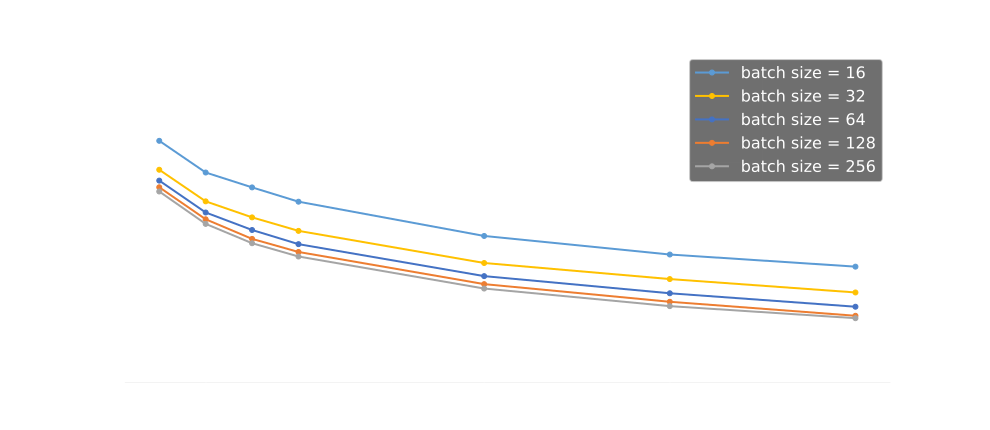
\includegraphics[width=1.0\textwidth]{scaling-a100}


\end{column}
\end{columns}

\end{frame}
\note{
}

%%%%%%%%%%%%%%%%%%%%%%%%%%%%%%%%%%%%%%%%%

\begin{frame}
\frametitle{Wrapping up}

\begin{columns}[T]
\begin{column}[T]{1.0\textwidth}
\setlength{\parskip}{0.5em}

\vspace{0.0cm}
\begin{enumerate}
\setlength{\parskip}{0.5em}
\item Converting code for distributed training is doable
\item Review and try out the batch scripts
\item More examples in the {\tt hpc-landscapes} repository
\end{enumerate}

\vspace{0.5cm}
\qquad \url{https://github.com/alan-turing-institute/hpc-landscape}

\end{column}
\end{columns}

\end{frame}
\note{
}


%%%%%%%%%%%%%%%%%%%%%%%%%%%%%%%%%%%%%%%%%%

\end{document}
